\documentclass[11pt,english]{article}

\usepackage[margin=1in]{geometry}
\usepackage{times}
\usepackage{microtype}
\usepackage{amsmath,amssymb,amsthm}
\usepackage{booktabs}
\usepackage{graphicx}
\usepackage{hyperref}
\usepackage{algorithm}
\usepackage{algpseudocode}
\usepackage{enumitem}
\usepackage{caption}
\usepackage[absolute, overlay]{textpos}
\usepackage{tikz}
\usepackage{array}
\usepackage{mathtools}
\usepackage{tcolorbox}
\tcbuselibrary{skins,breakable}
\usepackage{pdflscape}
\usepackage{rotating}
\usepackage{authblk}
\usepackage{multicol}


\usetikzlibrary{
	arrows.meta,
	positioning,
	calc,
	fit,
	backgrounds
}


\newtheorem{theorem}{Theorem}
\newtheorem{lemma}{Lemma}
\newtheorem{proposition}{Proposition}
\newtheorem{corollary}{Corollary}
\theoremstyle{remark}
\newtheorem{remark}{Remark}


\newcommand{\W}{\mathcal{W}}
\newcommand{\M}{\mathcal{M}}
\newcommand{\Uop}{\mathcal{U}}
\newcommand{\Gop}{\mathcal{G}}
\newcommand{\phitopo}{\phi_{\mathrm{topo}}}
\newcommand{\Score}{\mathrm{Score}}
\newcommand{\TopK}{\mathrm{TopK}}
\newcommand{\Sim}{\mathrm{Sim}}
\newcommand{\TimeGate}{\mathrm{TimeGate}}
\newcommand{\Merge}{\mathrm{Merge}}
\newcommand{\Gain}{\mathrm{Gain}}
\newcommand{\Cost}{\mathrm{Cost}}
\newcommand{\Novel}{\mathrm{Novel}}
\newcommand{\Unc}{\mathrm{Unc}}
\newcommand{\Gen}{\mathrm{Gen}}
\newcommand{\diag}{\mathrm{diag}}

\title{\textbf{MALAR}: Multi-scale Adaptive Learning with Abstraction and Recall\\
\large A general-purpose temporal learning model over scale-dependent graphs with topological memory}

\date {\today}

\begin{document}
\maketitle

\begin{abstract}
MALAR is a general-purpose learning framework for real-world systems whose observations are multidimensional,
scale-dependent, and temporally evolving. MALAR represents the world as a collection of coupled graphs and
higher-order complexes, computes objective and value fields that drive automated exploration and intervention,
and compresses learned structure into a time-stamped memory graph. Instead of storing raw trajectories,
MALAR stores compact graph and topological signatures (including persistent-homology summaries) together with
importance weights and learned timestamps. Memory entries are updated when novelty, change, or predicted goal
gain exceeds a threshold, and are retrieved by similarity plus temporal gating for both forward decision support
and reverse generation of plausible world states. We provide a unified mathematical formulation, an all-in-one
algorithm, comparisons to existing continual learning and memory-augmented models, and applied the suitability of MALAR for example use cases but not limited to these use cases: (i) multi-modal monitoring and screening for infectious disease in airport arrival environments using biological
sensor arrays (ii) a general industrial digital-twin setting (illustrative) where multi-scale
sensor graphs and topology drive closed-loop optimization.
\end{abstract}

\paragraph{Keywords.} continual learning; memory-augmented learning; topological data analysis; persistent homology; graph neural networks; active learning; temporal representation; anomaly detection.

\newpage
\begin{figure}[t]
	\centering
	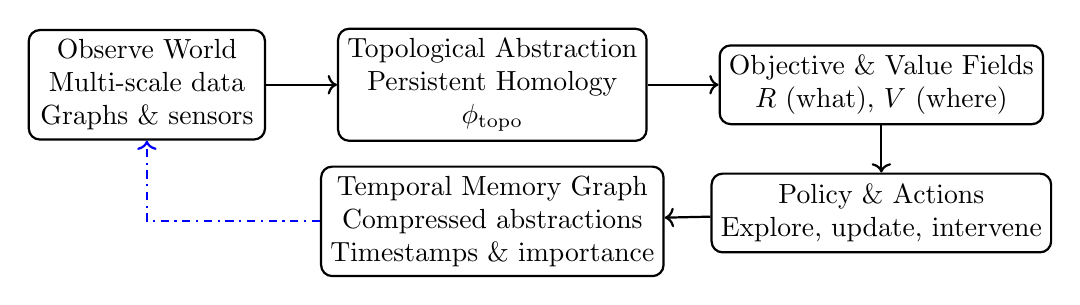
\begin{tikzpicture}[
		box/.style={draw, rounded corners, thick, minimum width=3.0cm, minimum height=1.0cm, align=center},
		arrow/.style={->, thick}
		]
		
		\node[box] (observe) {
			Observe World\\
			Multi-scale data\\
			Graphs \& sensors
		};
		
		\node[box, right=0.9cm of observe] (abstract) {
			Topological Abstraction\\
			Persistent Homology\\
			$\phi_{\mathrm{topo}}$
		};
		
		\node[box, right=0.9cm of abstract] (prioritize) {
			Objective \& Value Fields\\
			$R$ (what), $V$ (where)
		};
		
		\node[box, below=0.6cm of prioritize] (act) {
			Policy \& Actions\\
			Explore, update, intervene
		};
		
		\node[box, below=0.3cm of abstract] (memory) {
			Temporal Memory Graph\\
			Compressed abstractions\\
			Timestamps \& importance
		};
		
		\draw[arrow] (observe) -- (abstract);
		\draw[arrow] (abstract) -- (prioritize);
		\draw[arrow] (prioritize) -- (act);
		\draw[arrow] (act) -- (memory);
		\draw[arrow,dash dot,color=blue] (memory) -| (observe);
		
	\end{tikzpicture}
	\caption*{\textbf{Graphical Abstract.} MALAR is a general-purpose learning system that observes multi-scale worlds and prioritizes learning via objective and value fields, acts autonomously, and stores compact temporal memory for recall}
\end{figure}


\newpage
\maketitle
\section{Introduction}
Many real-world learning problems are not independent and identically distributed datasets but evolving systems: sensors drift, new regimes appear,
operating conditions change, and the scale at which structure matters may shift over time. Standard deep learning
pipelines store parameters but not the structured knowledge needed to detect regime shifts, compare with historical
patterns, and recover or simulate plausible prior states. MALAR addresses this by combining (a) a multi-scale structured
world representation; (b) distributed objective and value fields for prioritization; and (c) an explicit temporal memory
graph storing compressed topological and graph features with learned timestamps and importance weights.

\paragraph{Contributions.}
\begin{itemize}[leftmargin=1.3em]
\item A unified, domain-independent formulation for learning over multi-scale graphs and complexes.
\item Time-stamped topological memory: compressed graph/persistent-homology features stored and updated under novelty/goal-gain triggers.
\item A single all-in-one algorithm integrating observation, abstraction, prioritization, action selection, memory update, and recall/generation.
\item Comparison table vs.\ major families of memory-augmented and continual learning frameworks.
\item Two application sections including airport bio-sensing.
\end{itemize}

\section{Related Work}
MALAR intersects continual learning and replay, memory-augmented neural networks, dynamic graph learning,
active learning, and topological data analysis (TDA). MALAR differs in its explicit combination of objective and
value fields defined on a structured world, plus a compressed time-aware memory graph that stores topological
signatures rather than raw samples, enabling both similarity-based recall and reverse world-state generation.

\section{The MALAR Model}
\subsection{World as multi-scale temporal graphs and complexes}
Let the world at time $t$ be represented as a structured object
\begin{equation}
W(t) = (I, E(t), C(t), L(t)), \qquad u_i(t)\in \mathbb{R}^{d_u},
\end{equation}
where $I$ indexes locations/entities, $E(t)$ are edges, $C(t)$ are higher-order cells, and $L(t)$ denotes diffusion operators
(graph Laplacians and/or Hodge Laplacians).

\begin{figure}[t]
	\centering
	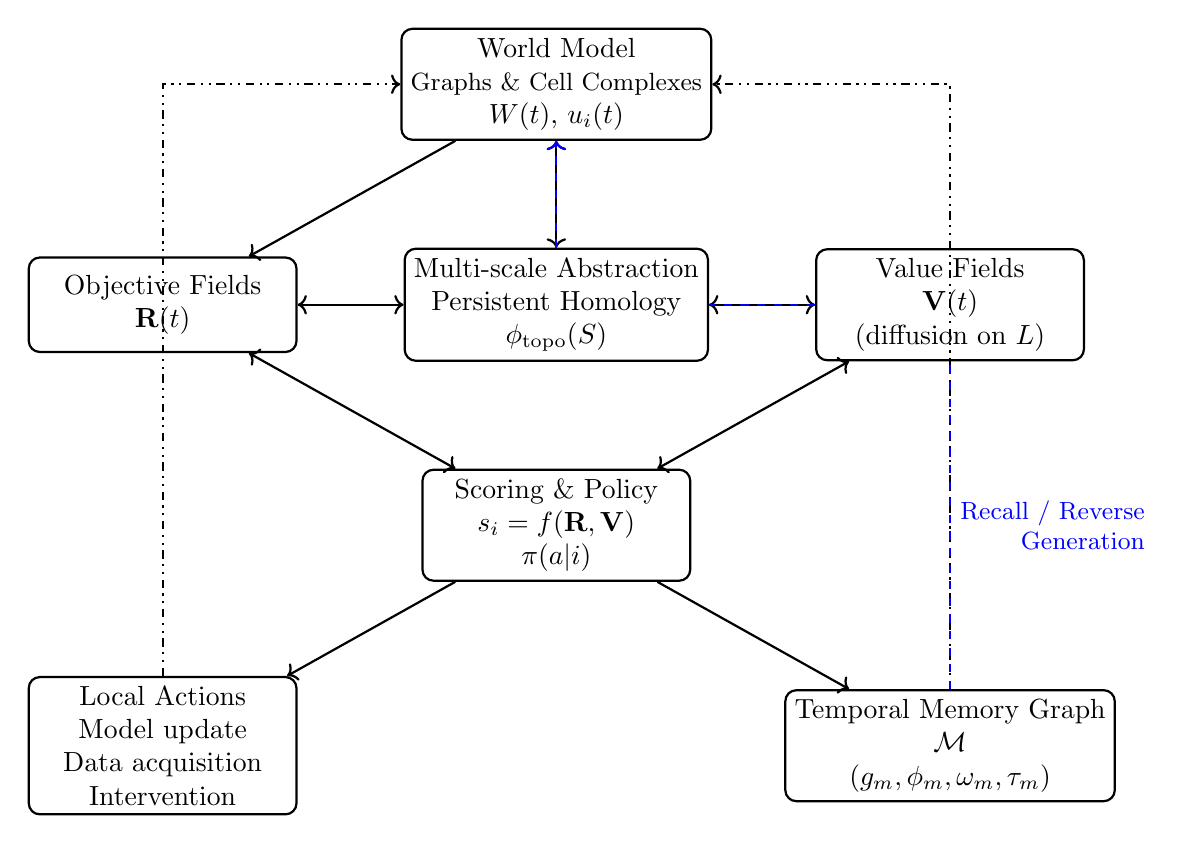
\begin{tikzpicture}[
		box/.style={draw, rectangle, rounded corners, thick, align=center, minimum width=3.4cm, minimum height=1.2cm},
		smallbox/.style={draw, rectangle, rounded corners, thick, align=center, minimum width=2.8cm, minimum height=1.0cm},
		arrow/.style={->, thick}
		]
		
		% --- Top row ---
		\node[box] (world) at (3,4.2)
		{World Model \\ \small Graphs \& Cell Complexes \\ $W(t)$, $u_i(t)$};
		
		\node[box] (topology) at (3,1.4)
		{Multi-scale Abstraction \\ Persistent Homology \\ $\phi_{\text{topo}}(S)$};
		
		% --- Middle row ---
		\node[box] (objective) at (-2.0,1.4)
		{Objective Fields \\ $\mathbf{R}(t)$};
		
		\node[box] (value) at (8.0,1.4)
		{Value Fields \\ $\mathbf{V}(t)$ \\ (diffusion on $L$)};
		
		% --- Scoring ---
		\node[box] (score) at (3,-1.4)
		{Scoring \& Policy \\ $s_i = f(\mathbf{R},\mathbf{V})$ \\ $\pi(a|i)$};
		
		% --- Bottom row ---
		\node[box] (actions) at (-2.0,-4.2)
		{Local Actions \\ Model update \\ Data acquisition \\ Intervention};
		
		\node[box] (memory) at (8,-4.2)
		{Temporal Memory Graph \\ $\mathcal{M}$ \\ $(g_m,\phi_m,\omega_m,\tau_m)$};
		
		% --- Arrows ---
		\draw[arrow,<->] (world) -- (topology);
		\draw[arrow] (world) -- (objective);
		\draw[arrow,<->] (topology) -- (objective);
		\draw[arrow,<->] (topology) -- (value);
		
		\draw[arrow,<->] (objective) -- (score);
		\draw[arrow,<->] (value) -- (score);
		
		\draw[arrow] (score) -- (actions);
		\draw[arrow] (score) -- (memory);
		
		\draw[arrow,dash dot dot] (actions) |- (world);
		\draw[arrow,dash dot dot] (memory) |- (world);
		
		% --- Memory recall arrow ---
	    \draw[arrow,dashed,color=blue] (memory) -- node[right,align=right, font=\small]
	 	{Recall / Reverse \\ Generation}
		(value) -- (topology) -- (world);
		
	\end{tikzpicture}
	\caption{MALAR: Multi-scale Adaptive Learning with Abstraction and Recall. The system observes a structured world, extracts multi-scale topological abstractions, computes objective and value fields, selects actions under resource constraints, and stores compressed knowledge in a temporal memory graph enabling recall and reverse generation.}
	\label{fig:malar-overview}
\end{figure}

\subsection{Objective and value fields}
MALAR maintains $K$ objective fields and $M$ value fields:
\begin{equation}
R_i(t) = (R_i^{(1)}(t),\dots,R_i^{(K)}(t)), \qquad
V_i(t) = (V_i^{(1)}(t),\dots,V_i^{(M)}(t)).
\end{equation}
Values propagate across structure via diffusion with sources:
\begin{equation}
V(t+\Delta t) = V(t) - \Delta t\, L(t)V(t) + \Delta t\, S_V(u(t),R(t)).
\end{equation}


\subsection{Topological abstraction and compression}
For regions $S$ (subgraphs/subcomplexes) and layers $r\in\{1,\dots,R\}$, MALAR builds filtrations and computes
persistence diagrams $D_{r,S}^{(d)}$. These are embedded into vectors $\phi_r(S)$ and concatenated:
\begin{equation}
\phi_{\text{topo}}(S) = [\phi_1(S)\,\Vert\,\phi_2(S)\,\Vert\,\dots\,\Vert\,\phi_R(S)].
\end{equation}

\begin{figure}[t]
	\centering
	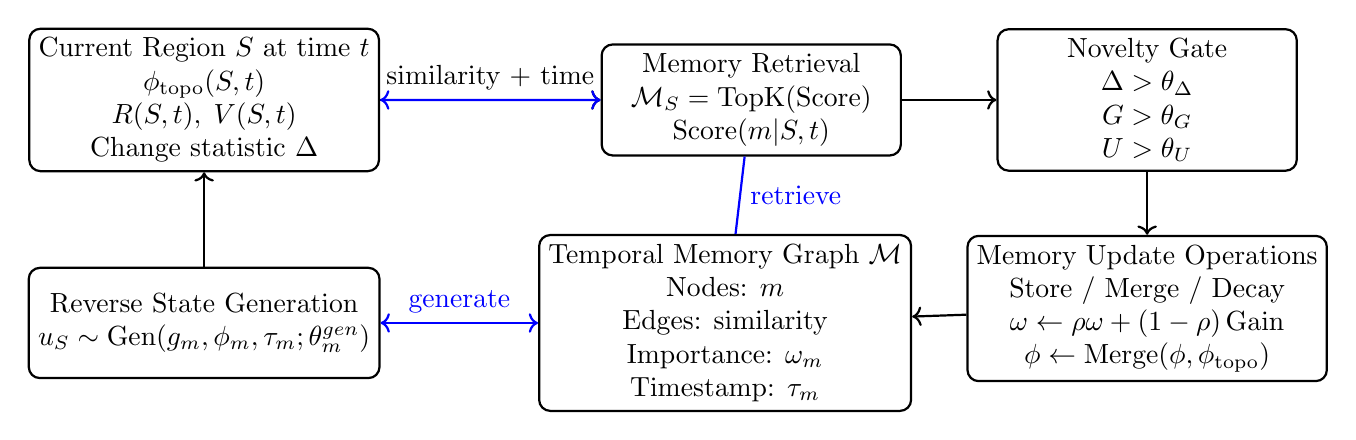
\begin{tikzpicture}[
		box/.style={draw, rounded corners, thick, align=center, minimum width=3.8cm, minimum height=1.4cm},
		smallbox/.style={draw, rounded corners, thick, align=center, minimum width=3.4cm, minimum height=1.1cm},
		arrow/.style={->, thick},
		node distance=1.6cm
		]
		
		% Nodes
		\node[box] (current) {
			Current Region $S$ at time $t$\\
			$\phi_{\mathrm{topo}}(S,t)$\\
			$R(S,t),\;V(S,t)$\\
			Change statistic $\Delta$
		};
		
		\node[box, right=2.8cm of current] (retrieve) {
			Memory Retrieval\\
			$\mathcal{M}_S = \mathrm{TopK}(\mathrm{Score})$\\
			$\mathrm{Score}(m|S,t)$
		};
		
		\node[box, right=1.2cm of retrieve] (gate) {
			Novelty Gate\\
			$\Delta > \theta_\Delta$\\
			$G > \theta_G$\\
			$U > \theta_U$
		};
		
		\node[box, below=0.8cm of gate] (update) {
			Memory Update Operations\\
			Store / Merge / Decay\\
			$\omega \leftarrow \rho \omega + (1-\rho)\,\mathrm{Gain}$\\
			$\phi \leftarrow \mathrm{Merge}(\phi,\phi_{\mathrm{topo}})$
		};
		
		\node[box, below=1.2cm of current] (reverse) {
			Reverse State Generation\\
			$u_S \sim \mathrm{Gen}(g_m,\phi_m,\tau_m;\theta_m^{gen})$
		};
		
		\node[box, right=2.0cm of reverse] (memory) {
			Temporal Memory Graph $\mathcal{M}$\\
			Nodes: $m$\\
			Edges: similarity\\
			Importance: $\omega_m$\\
			Timestamp: $\tau_m$
		};
		
		
		
		% Arrows
		\draw[arrow] (current) -- node[above]{similarity + time} (retrieve);
		\draw[arrow] (retrieve) -- (gate);
		\draw[arrow] (gate) -- (update);
		\draw[arrow] (update) -- (memory);
		\draw[arrow,<->,color=blue] (memory) -- node[right]{retrieve} (retrieve) -- (current);
		\draw[arrow,<->,color=blue] (memory) -- node[above]{generate} (reverse);
		\draw[arrow] (reverse) -- (current);
		
	\end{tikzpicture}
	\caption{
		\textbf{Memory-centric MALAR architecture.}
		Current multi-scale abstractions are compared against a temporal memory graph using similarity and time-gated retrieval.
		Novelty, uncertainty, or goal gain triggers memory insertion or merge; otherwise entries decay.
		Stored memory supports both forward decision support and reverse world-state generation.
	}
	\label{fig:malar-memory}
\end{figure}

\subsection{Temporal memory graph with learned timestamps}
MALAR stores compressed information in a temporal memory graph $\mathcal{M}$. Each memory item $m$ stores:
\begin{equation}
m = (g_m, \phi_m, \omega_m, \tau_m, \theta_m^{gen}),
\end{equation}
where $g_m$ is a compact graph/complex abstraction, $\phi_m$ is a topological descriptor, $\omega_m$ is importance,
$\tau_m$ is a learned real-world timestamp, and $\theta_m^{gen}$ parameterizes optional reverse generation.



\section{Learning, Recall, and Generation}
\subsection{Comparing current state to memory}
For region $S$ at time $t$, MALAR retrieves memory by similarity and temporal gating:
\begin{equation}
\text{Score}(m\mid S,t) = \text{Sim}(\phi_{\text{topo}}(S,t),\phi_m) + \lambda\,\text{TimeGate}(t,\tau_m) + \mu\,\omega_m.
\end{equation}
Low score or high change indicates novelty and triggers insertion/merge.

\subsection{Memory update rule}
Let $\Delta$ be a change statistic (e.g.\ PH distance, embedding distance) and $G$ predicted goal gain. Store if:
\begin{equation}
\Delta > \theta_\Delta \quad \text{or}\quad G>\theta_G \quad \text{or}\quad \text{Uncertainty}(S)>\theta_U.
\end{equation}
Otherwise update via importance-weighted merging/decay:
\begin{equation}
\omega_m \leftarrow \rho\,\omega_m + (1-\rho)\,\text{Gain}(S),\qquad
\phi_m \leftarrow \text{Merge}(\phi_m,\phi_{\text{topo}}(S)).
\end{equation}



\subsection{Reverse world-state generation}
MALAR supports reverse generation by attaching $\theta_m^{gen}$ to memory items:
\begin{equation}
p(u_S\mid m) = \text{Gen}(u \mid g_m,\phi_m,\tau_m;\theta_m^{gen}).
\end{equation}

\begin{algorithm}[t]
	\caption{MALAR (Multi-scale Adaptive Learning with Abstraction and Recall)}
	\begin{algorithmic}[1]
		\State \textbf{Input:} initial world $W(0)$, states $u(0)$, memory $\mathcal{M}\leftarrow \emptyset$, budgets $B$, thresholds $\Theta$
		\For{$t=0,1,2,\dots$}
		\State Observe data; $W(t)\leftarrow \textsc{UpdateWorld}(W(t),\text{data}_t)$
		\State $u(t)\leftarrow F_{\text{rep}}(u(t),W(t))$
		\ForAll{regions $S\leftarrow \textsc{RegionSampler}(W(t),B)$}
		\State $\phi_{\text{topo}}(S,t)\leftarrow \textsc{TopologyEncode}(W(t),u(t),S)$
		\State $R(S,t)\leftarrow \textsc{ComputeObjectives}(W(t),u(t),S)$
		\State $V(S,t)\leftarrow \textsc{DiffuseAndSourceValues}(W(t),u(t),R,S)$
		\State $\mathcal{M}_S \leftarrow \textsc{Retrieve}(\mathcal{M},\phi_{\text{topo}}(S,t),t)$
		\State $\Delta \leftarrow \textsc{ChangeStat}(\phi_{\text{topo}}(S,t),\mathcal{M}_S)$
		\If{\textsc{Novel}$(\Delta,R,V)$} $\mathcal{M}\leftarrow \textsc{StoreOrMerge}(\mathcal{M},S,\phi_{\text{topo}}(S,t),R,V,t)$ \EndIf
		\State $s(S)\leftarrow \textsc{ScoreRegion}(R(S,t),V(S,t),\textsc{Cost}(S))$
		\EndFor
		\State Select top regions $S^\star$ under budget; for each $S^\star$ choose action $a\sim \pi(a\mid u,R,V,\mathcal{M}_{S^\star})$
		\State Execute: $(u,W,\mathcal{M}) \leftarrow \textsc{Execute}(a,S^\star,u,W,\mathcal{M})$
		\State $\mathcal{M}\leftarrow \textsc{CompressAndDecay}(\mathcal{M})$
		\EndFor
	\end{algorithmic}
\end{algorithm}

\section{All-in-one Algorithm}

MALAR operates on four core ideas (Algorithm 1):
\begin{itemize}
\item Structured World Representation : The world is represented as evolving graphs and cell complexes.

\item Objective and Value Fields : Learning is guided by spatially distributed fields: Objective fields: What is good? Value fields : Where does learning matter most?

\item Topological and Spectral Abstraction : Persistent, scale-invariant structures are extracted using topology and spectral operators.

\item Memory as a Compressed Graph : Only compressed, objective-relevant abstractions are stored in a temporal memory graph.

\end{itemize}

\section{Comparison to Existing Frameworks}

Unlike existing paradigms, MALAR integrates multi-scale structural representations,
explicit time-aware memory, and topological abstraction within a single closed-loop
learning framework. Objective and value fields are separated and diffused over structured
world graphs, enabling autonomous exploration, temporal recall, and reverse world-state
generation. A comparison with existing state of the art learning models are given in Table 1.


\begin{figure}[t]
	\centering
	\begin{tikzpicture}[
		box/.style={draw, rectangle, rounded corners, thick, align=center, minimum width=3.4cm, minimum height=1.2cm},
		overlay/.style={draw, dashed, rounded corners, thick, align=left, inner sep=6pt},
		arrow/.style={->, thick},
		node distance=1.0cm
		]
		
		% Backbone
		\node[box] (world)  at (-6.2,4) {World Graph $W(t)$} ;
		\node[box] (topo) at (1.2,4) {Topological Abstraction\\ $\phi_{\mathrm{topo}}$};
		\node[box] (fields) at (8.2,4) {Objective \& Value Fields\\ $R(t), V(t)$};
		\node[box] (memory) at (8.2,1.8) {Temporal Memory\\ $\mathcal{M}$};
		
		\node[box, below=of topo, minimum width=6.5cm] (policy) {
			Policy \& Actions\\
			$\pi(a|S,t)$ \quad $\mathcal{U}$ (local) \quad $\mathcal{G}$ (global)
		};
		
		% Arrows backbone
		\draw[arrow] (world) -- (topo);
		\draw[arrow] (topo) -- (fields);
		\draw[arrow] (fields) -- (memory);
		\draw[arrow] (fields) -- (policy);
		\draw[arrow] (memory) -- (policy);
		\draw[arrow] (policy) -| (world);
		
		% Overlay A
		\node[overlay, below left=1.0cm and -1.0cm of policy, text width=6.4cm] (overlayA) {
			\textbf{Overlay A: Airport Infectious-Disease Monitoring}\\
			Nodes: zones, sensors, queues, airflow paths\\
			Edges: adjacency, airflow, human flow\\
			Objectives: early detection, false-positive control\\
			Values: anomaly, uncertainty, public-health impact\\
			Memory: seasonal baselines, outbreak signatures
		};
		
		% Overlay B
		\node[overlay, below right=1.0cm and -5.0cm of policy, text width=6.4cm] (overlayB) {
			\textbf{Overlay B: Industrial Digital Twin (Generic)}\\
			Nodes: assets, process steps, sensors, QA points\\
			Edges: dependencies, material flow\\
			Objectives: quality, yield, safety\\
			Values: leverage, uncertainty, risk\\
			Memory: operating regimes, faults, recipes
		};
		
		% Overlay arrows
		\draw[arrow, dashed,color=blue] (overlayA.north) -| (world.south);
		\draw[arrow, dashed,color=blue] (overlayB.north) -| (world.south);
		
	\end{tikzpicture}
	\caption{
		\textbf{Application-specific overlays.}
		The same MALAR backbone is instantiated with domain-specific world graphs, objective/value fields,
		and memory semantics. Shown examples include airport bio-sensing with Raman spectroscopy and a generic industrial digital-twin setting.
	}
	\label{fig:malar-overlays}
\end{figure}


\section{Applications}
\subsection{Airport infectious-disease monitoring with biological sensors}
MALAR can be deployed as an adaptive monitoring system in airport arrival/immigration/baggage halls. Inputs may include
heterogeneous sensor arrays (air-quality, aerosol particle counters, VOC sensors, biosensors, thermal kiosks, environmental
metadata) plus spectroscopy stations for rapid biochemical signatures. The world $W(t)$ is a spatio-temporal graph over
zones and sensor nodes, with edges encoding airflow and human-flow coupling. Objective fields encode screening goals
(early outbreak detection, false-positive control, throughput constraints), while value fields prioritize sampling and
model refinement (zones with uncertainty, anomalous spectroscopy signatures, high predicted public-health impact). MALAR’s memory
stores compressed multi-modal graph/topology signatures of past regimes (seasonal baselines, outbreak patterns, sensor drift)
with timestamps enabling rapid comparison and baseline generation for change detection.

\subsection{Industrial digital-twin optimization (illustrative)}
In industrial settings, MALAR serves as a self-learning digital twin fusing process, sensors, inspection, and performance.
Value diffusion prioritizes experiments and sensor placement, while memory stores regime abstractions (normal, drift, faults)
for diagnosis and counterfactual simulation.


\begin{table}[t]
\centering
\caption{Comparison of MALAR to representative families of approaches.}
\begin{tabular}{p{2.6cm}p{2.6cm}p{2.2cm}p{2.2cm}p{1.6cm}p{3.2cm}}
\toprule
Family & Core idea & Memory type & Temporal handling & Topology-aware? & MALAR difference \\
\midrule
Replay-based continual learning & store/replay samples & raw samples & implicit & no & compressed graph+topology; explicit timestamps; recall+generation \\
Memory-augmented nets (NTM/DNC) & differentiable memory & key-value vectors & implicit & no & memory is a graph of abstractions; importance + timestamp; diffusion fields \\
Dynamic graph learning & temporal GNNs & embeddings & yes & sometimes & adds objective/value fields + novelty gating + topological compression \\
Active learning/Bayesian opt. & query uncertainty & none & limited & no & uncertainty as value field; stores multi-scale abstractions over time \\
TDA-based ML & topological descriptors & vectors & rare & yes & integrates PH into time-aware memory with update/merge/decay and closed-loop actions \\
\bottomrule
\end{tabular}
\end{table}


\section{Discussion and Limitations}
Strengths include explicit structural representation, topology-aware compression, and time-aware memory update.
Limitations include computational cost of streaming topology, robust region sampling/registration, and design choices for memory
merge/decay. Future work includes regret bounds under non-stationarity, efficient streaming PH, and tighter integration of
generative memory with action policies. A comparison of the MALAR with families of different approach are given in table 2.

\begin{table}[t]
	\centering
	\caption{Comparison of MALAR with major learning paradigms. 
		Symbols: \checkmark = supported, \checkmark\checkmark = strongly supported, 
		$\triangle$ = partial/implicit, $\times$ = not supported.}
	\label{tab:comparison}
	\begin{tabular}{lcccccc}
		\toprule
		\textbf{Feature} 
		& \textbf{Deep Learning} 
		& \textbf{RL} 
		& \textbf{Continual Learning} 
		& \textbf{GNNs} 
		& \textbf{World Models} 
		& \textbf{MALAR} \\
		\midrule
		Multi-scale structure            & $\times$ & $\times$ & $\times$ & $\triangle$ & $\triangle$ & \textbf{\checkmark} \\
		Explicit memory                  & $\times$ & $\triangle$ & \checkmark & $\times$ & $\triangle$ & \textbf{\checkmark\checkmark} \\
		Topological abstraction          & $\times$ & $\times$ & $\times$ & $\times$ & $\times$ & \textbf{\checkmark} \\
		Objective / value separation     & $\times$ & \checkmark & $\times$ & $\times$ & $\times$ & \textbf{\checkmark} \\
		Temporal recall                  & $\times$ & $\triangle$ & $\triangle$ & $\times$ & $\triangle$ & \textbf{\checkmark\checkmark} \\
		Reverse state generation         & $\times$ & $\times$ & $\times$ & $\times$ & \checkmark & \textbf{\checkmark\checkmark} \\
		Autonomous exploration           & $\times$ & \checkmark & $\times$ & $\times$ & $\triangle$ & \textbf{\checkmark} \\
		\bottomrule
	\end{tabular}
\end{table}

\section{Conclusion}
MALAR is an all-in-one model for continual learning over multi-scale structured worlds. By combining objective/value fields
with topology-aware temporal memory, MALAR supports automated exploration, change detection, recall, and reverse generation.

\bibliographystyle{plain}
\begin{thebibliography}{9}
	\bibitem{tda} Edelsbrunner and Harer. \emph{Computational Topology}. AMS, 2010.
	\bibitem{gnn} Wu et al. A comprehensive survey on graph neural networks. \emph{IEEE TNNLS}, 2021.
	\bibitem{cl} Parisi et al. Continual lifelong learning with neural networks. \emph{Neural Networks}, 2019.
\end{thebibliography}

\newpage
\appendix
\section{Appendix : Mathematical Details and Proof Sketches}
\subsection{Operators}
Graph Laplacian $L = D-A$. For cell complexes, Hodge Laplacians are
$L_0=B_1B_1^\top$, $L_1=B_1^\top B_1 + B_2B_2^\top$, $L_2=B_2^\top B_2$.
MALAR uses these to diffuse value fields.

\subsection{Change statistics}
Let $D$ and $D'$ be persistence diagrams. Define $\Delta_{PH}=d_{PH}(D,D')$ using bottleneck or Wasserstein distance.
For embeddings $\phi$, use $\Delta=\|\phi-\phi'\|_2$ or cosine distance.

\subsection{Memory update as budgeted utility}
Memory update can be framed as maximizing retained utility $U(\mathcal{M})$ subject to budget $\sum_{m\in\mathcal{M}} c(m)\le B$.
Thresholded insertion and merge/decay approximate greedy selection.

\subsection{Proof sketches}
\paragraph{Stability of diffusion.} For explicit Euler $V\leftarrow V-\Delta t\,LV$, stability holds for $\Delta t < 2/\lambda_{\max}(L)$,
by spectral decomposition.

\begin{theorem}[Stability of explicit value diffusion]
	\label{thm:diffusion-stability}
	Let $L$ be a symmetric positive semidefinite operator (e.g.\ a graph Laplacian or Hodge Laplacian) with eigenvalues
	$0=\lambda_1\le \cdots \le \lambda_{\max}$. Consider the explicit update
	\[
	V^{t+1} = V^t - \Delta t\, L V^t + \Delta t\, S^t,
	\]
	where $S^t$ is any bounded source term. If $0<\Delta t < \frac{2}{\lambda_{\max}}$, then the homogeneous part
	$V^{t+1}= (I-\Delta t\,L)V^t$ is non-expansive in $\ell_2$ (spectral radius $\le 1$), and the full system is stable
	in the sense that $\|V^t\|_2$ remains bounded for bounded $\{S^t\}$.
\end{theorem}

\begin{proof}[Proof sketch]
	Diagonalize $L=Q\Lambda Q^\top$. The homogeneous iteration is $V^{t+1}=Q(I-\Delta t\,\Lambda)Q^\top V^t$.
	Stability requires $|1-\Delta t\,\lambda_k|\le 1$ for all $k$, equivalent to $0\le \Delta t\,\lambda_k \le 2$.
	Thus $\Delta t <2/\lambda_{\max}$. Bounded forcing follows by standard linear system bounds.
\end{proof}


\paragraph{EMA importance boundedness.} If $\omega\leftarrow \rho\omega+(1-\rho)g_t$ with $g_t\ge 0$, then $\omega$ remains nonnegative and bounded
by $\sup_t g_t$.

\begin{theorem}[Convergence of importance weights under stationary gains]
	\label{thm:ema-convergence}
	Let a memory item $m$ have importance update
	\[
	\omega_{t+1} = \rho\,\omega_t + (1-\rho)\,g_t,
	\qquad 0<\rho<1,
	\]
	where $g_t$ is the instantaneous gain assigned to the memory item at time $t$.
	(i) If $g_t \equiv g$ is constant, then $\omega_t \to g$ as $t\to\infty$.
	(ii) If $g_t$ is bounded, then $\{\omega_t\}$ is bounded and satisfies
	$\omega_t = (1-\rho)\sum_{k=0}^{t-1}\rho^{k}g_{t-1-k}+\rho^t\omega_0$.
\end{theorem}

\begin{proof}[Proof sketch]
	Unroll the recursion to obtain the closed form. For constant $g$, the geometric series gives $\omega_t-g=\rho^t(\omega_0-g)\to 0$.
\end{proof}


\paragraph{Greedy approximation.} Under submodularity assumptions for $U(\mathcal{M})$ and uniform costs, greedy achieves a $(1-1/e)$ approximation.
Formal guarantees require establishing submodularity for the chosen utility on compressed descriptors.

\begin{theorem}[Memory dictionary convergence under stable regimes and strict novelty thresholds]
	\label{thm:memory-dictionary}
	Assume the environment enters a regime after time $T_0$ where regional descriptors $\phitopo(S,t)$
	belong to a compact set $\mathcal{K}$ and satisfy a Lipschitz temporal variation bound:
	$\|\phitopo(S,t+1)-\phitopo(S,t)\|\le \varepsilon$ for all $t\ge T_0$.
	If MALAR inserts new memory items only when the novelty statistic
	$\Delta(S,t)\ge \theta_\Delta$ with $\theta_\Delta > \varepsilon$, and merge operations are contractive
	(e.g.\ $\|\Merge(\phi,\phi')-\phi\|\le c\|\phi'-\phi\|$ with $0<c<1$),
	then the number of memory insertions after $T_0$ is finite, and the memory graph stabilizes up to bounded merge updates.
\end{theorem}

\begin{proof}[Proof sketch]
	After $T_0$, successive descriptors differ by at most $\varepsilon<\theta_\Delta$, so novelty-triggered insertions stop
	except possibly for a finite transient. Contractive merges produce a Cauchy-like stabilization of stored descriptors.
\end{proof}

\begin{remark}
	Theorem~\ref{thm:memory-dictionary} is a formalization of “no new memories once the world stops changing beyond the novelty threshold.”
	If the world is nonstationary, insertions may continue, but budgeted decay/compression keeps memory bounded.
\end{remark}



\newpage
\begin{figure}[t]
	\centering
	\title{Annexure B: Slide by side view of Algorithm and Mathematical model}
	\newline
	\begin{tcolorbox}[
		width=\textwidth,
		spread sidewards=-2.5cm,
		enhanced,
		colback=white,
		colframe=black,
		boxrule=1.0pt,
		arc=2mm,
		]
		
		\begin{minipage}[t]{0.45\linewidth}
			\textbf{MALAR: Implementation Skeleton (Algorithmic)}\\[8pt]
			
			\begin{algorithmic}[1]
				\State Initialize world $\W(0)$, states $u(0)$, memory $\M\leftarrow\emptyset$, budgets $B$, thresholds $\Theta$
				\For{$t=0,1,2,\dots$}
				\State $\W(t)\leftarrow \mathrm{UpdateWorld}(\W(t),\mathrm{data}_t)$
				\State $u(t)\leftarrow F_{\mathrm{rep}}(u(t),\W(t))$
				\ForAll{regions $S \leftarrow \mathrm{RegionSampler}(\W(t),B)$}
				\State $\phitopo(S,t)\leftarrow \mathrm{TopologyEncode}(\W(t),u(t),S)$
				\State $R(S,t)\leftarrow F_R(\W(t),u(t),S)$
				\State $V(S,t)\leftarrow \mathrm{DiffuseAndSource}(V,\W(t),u(t),R)$
				\State $\M_S\leftarrow \TopK\!\big(\Score(m\mid S,t)\big)$
				\State $\Delta\leftarrow \mathrm{ChangeStat}(\phitopo(S,t),\M_S)$
				\If{$\Novel(\Delta,R,V)$}
				\State $\M\leftarrow \mathrm{StoreOrMerge}(\M,S,\phitopo,R,V,t)$
				\EndIf
				\State $s(S,t)\leftarrow \alpha^\top R(S,t)+\beta^\top V(S,t)-\gamma\,\Cost(S)$
				\EndFor
				\State Select top-$k$ regions $S^\star$ under budget
				\ForAll{$S \in S^\star$}
				\State Sample action $a \sim \pi(a\mid S,t)$
				\State Execute $(u,\W,\M)\leftarrow \Uop(S,a)$ or invoke $\Gop^{(q)}$ if triggered
				\EndFor
				\State $\M\leftarrow \mathrm{CompressAndDecay}(\M)$
				\EndFor
			\end{algorithmic}
			
		\end{minipage}
		\hfill
		\begin{minipage}[t]{0.49\linewidth}
			\textbf{MALAR: Mathematical Formulation (Core)}\\[8pt]
			
			\textbf{World:}
			\[
			\W(t)=(I,E(t),C(t),L(t)),\quad u_i(t)\in\mathbb{R}^{d_u}.
			\]
			
			\textbf{Topology abstraction (region $S$):}
			\[
			\phitopo(S,t)=[\phi_1(S,t)\Vert\cdots\Vert\phi_R(S,t)].
			\]
			
			\textbf{Fields:}
			\[
			R_i(t)\in\mathbb{R}^K,\quad V_i(t)\in\mathbb{R}^M.
			\]
			
			\textbf{Value propagation:}
			\[
			V(t+\Delta t)=V(t)-\Delta t\,L(t)V(t)+\Delta t\,S_V(u(t),R(t)).
			\]
			
			\textbf{Score:}
			\[
			s(S,t)=\alpha^\top R(S,t)+\beta^\top V(S,t)-\gamma\,\Cost(S).
			\]
			
			\textbf{Policy:}
			\[
			\pi(a\mid S,t)=\mathrm{softmax}_a(z_a(u,R,V,\M_S)/T).
			\]
			
			\textbf{Memory item:}
			\[
			m=(g_m,\phi_m,\omega_m,\tau_m,\theta^{gen}_m).
			\]
			
			\textbf{Retrieval:}
			\[
			\Score(m\mid S,t)=\Sim(\phitopo(S,t),\phi_m)+\lambda\TimeGate(t,\tau_m)+\mu\omega_m.
			\]
			
			\textbf{Novelty gate:}
			\[
			\Delta>\theta_\Delta\;\vee\;G>\theta_G\;\vee\;\Unc>\theta_U.
			\]
			
			\textbf{Generation:}
			\[
			u_S\sim \Gen(g_m,\phi_m,\tau_m;\theta^{gen}_m).
			\]
			
		\end{minipage}
		
	\end{tcolorbox}
	
	\caption{Parallel view: MALAR implementation (left) and mathematical core (right).}
	\label{fig:malar-parallel}
\end{figure}

\newpage

\begin{figure}[t]
	\centering
	\title{Annexure C: Hypothetical deployment model for MALAR in Infectious decease monitoring}
	\newline
	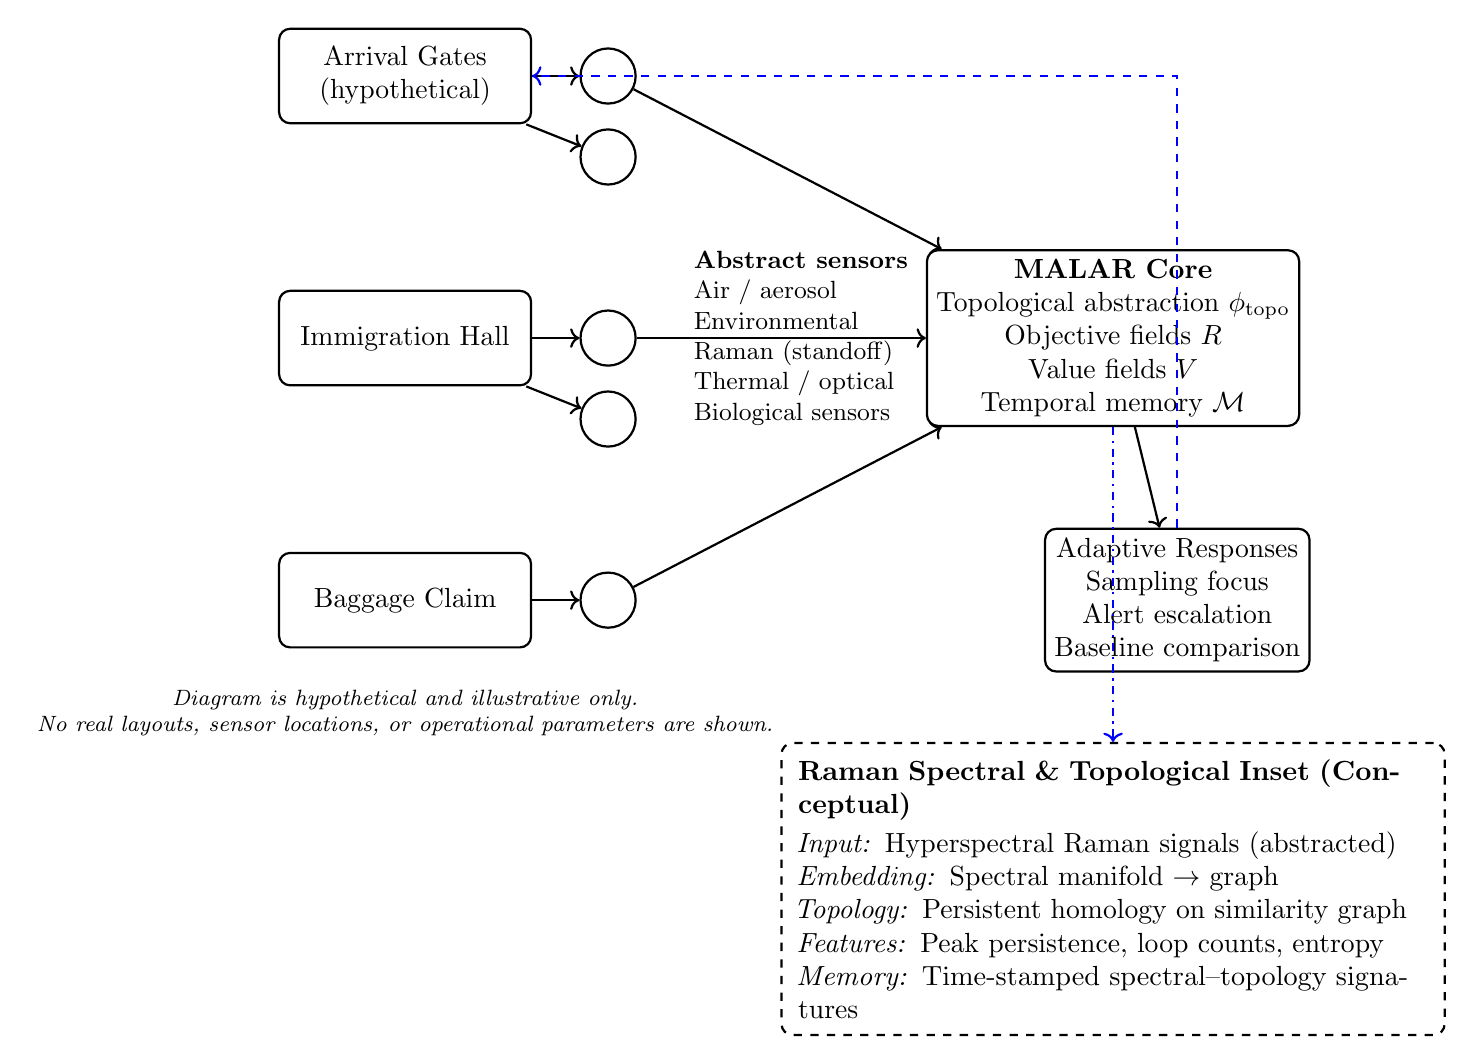
\begin{tikzpicture}[
		zone/.style={draw, rounded corners, thick, minimum width=3.2cm, minimum height=1.2cm, align=center},
		sensor/.style={draw, circle, thick, minimum size=0.7cm},
		malar/.style={draw, rounded corners, thick, minimum width=4.2cm, minimum height=1.4cm, align=center},
		inset/.style={draw, dashed, rounded corners, thick, inner sep=6pt},
		arrow/.style={->, thick}
		]
		
		% =========================
		% Airport zones (hypothetical)
		% =========================
		\node[zone] (arrival) at (-4.1,4) {Arrival Gates\\(hypothetical)};
		\node[zone, below=2.1cm of arrival] (immigration) {Immigration Hall};
		\node[zone, below=2.1cm of immigration] (baggage)  {Baggage Claim};
		
		% =========================
		% Sensor nodes (abstract)
		% =========================
		\node[sensor, right=0.6cm of arrival] (s1) {};
		\node[sensor, below=0.3cm of s1] (s2) {};
		\node[sensor, right=0.6cm of immigration] (s3) {};
		\node[sensor, below=0.3cm of s3] (s4) {};
		\node[sensor, right=0.6cm of baggage] (s5) {};
		
		\node[align=left, font=\small, right=0.6cm of s3] (slabel) {
			\textbf{Abstract sensors}\\
			Air / aerosol\\
			Environmental\\
			Raman (standoff)\\
			Thermal / optical \\
			Biological sensors
		};
		
		% =========================
		% MALAR core
		% =========================
		\node[malar, right=5.0cm of immigration] (malarcore) {
			\textbf{MALAR Core}\\
			Topological abstraction $\phi_{\mathrm{topo}}$\\
			Objective fields $R$\\
			Value fields $V$\\
			Temporal memory $\mathcal{M}$
		};
		
		% =========================
		% Action / response layer
		% =========================
		\node[zone, right=6.5cm of baggage] (action) {
			Adaptive Responses\\
			Sampling focus\\
			Alert escalation\\
			Baseline comparison
		};
		
		% =========================
		% Arrows: zones → sensors → MALAR
		% =========================
		\draw[arrow] (arrival) -- (s1);
		\draw[arrow] (arrival) -- (s2);
		\draw[arrow] (immigration) -- (s3);
		\draw[arrow] (immigration) -- (s4);
		\draw[arrow] (baggage) -- (s5);
		
		\draw[arrow] (s1) -- (malarcore);
		\draw[arrow] (s3) -- (malarcore);
		\draw[arrow] (s5) -- (malarcore);
		
		\draw[arrow] (malarcore) -- (action);
		\draw[arrow, dashed,color=blue] (action) |- (arrival);
		
		% =========================
		% Raman + topology inset
		% =========================
		\node[inset, below=4.0cm of malarcore, text width=8.0cm] (raman) {
			\textbf{Raman Spectral \& Topological Inset (Conceptual)}\\[2pt]
			\emph{Input:} Hyperspectral Raman signals (abstracted)\\
			\emph{Embedding:} Spectral manifold $\rightarrow$ graph\\
			\emph{Topology:} Persistent homology on similarity graph\\
			\emph{Features:} Peak persistence, loop counts, entropy\\
			\emph{Memory:} Time-stamped spectral–topology signatures
		};
		
		\draw[arrow, dash dot, color=blue] (malarcore) -- (raman);
		
		% =========================
		% Annotation
		% =========================
		\node[align=center, font=\footnotesize, below=0.4cm of baggage] {
			\textit{Diagram is hypothetical and illustrative only.}\\
			\textit{No real layouts, sensor locations, or operational parameters are shown.}
		};
		
	\end{tikzpicture}
	\caption{
		Hypothetical deployment of MALAR at international entry points. Abstract airport zones and sensor networks form a spatio-temporal world graph. MALAR performs topological abstraction, objective/value prioritization, and temporal memory updates. A conceptual Raman-spectral inset illustrates topology-aware feature extraction without exposing sensitive data.
	}
	\label{fig:malar-deployment}
\end{figure}

\newpage

\begin{figure}[t]
	\title{Annexure D:Hypothetical deployment of MALAR for Manufacturing digital twin}
	\newline
	
	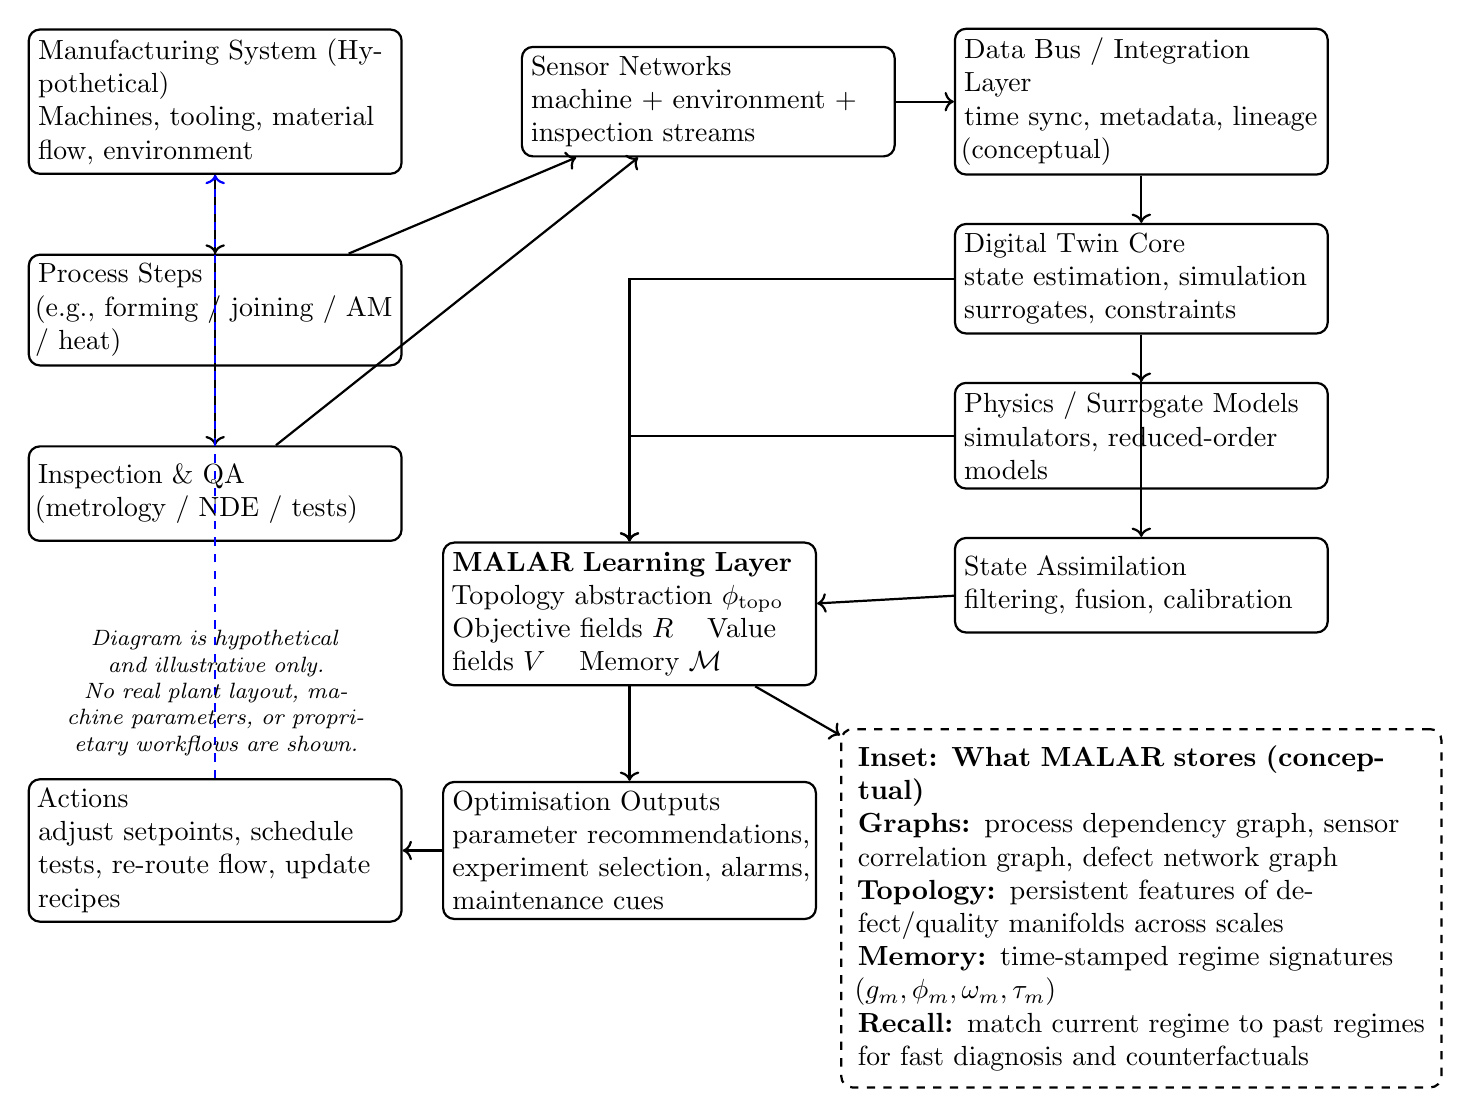
\begin{tikzpicture}[
		box/.style={draw, rounded corners, thick, align=left, minimum width=3.4cm, minimum height=1.2cm, text width=4.5cm},
		wide/.style={draw, rounded corners, thick, align=left, minimum width=6.8cm, minimum height=1.3cm},
		dashedbox/.style={draw, dashed, rounded corners, thick, align=left, inner sep=6pt},
		arrow/.style={->, thick},
		node distance=1.4cm
		]
		
		% =========================
		% Physical manufacturing line (hypothetical)
		% =========================
		\node[box] (plant) at (-4.1,4.2) {Manufacturing System (Hypothetical)\\ Machines, tooling, material flow, environment};
		\node[box, below=1.0cm of plant] (process) {Process Steps\\ (e.g., forming / joining / AM / heat)};
		\node[box, below=1.0cm of process] (qa) {Inspection \& QA\\ (metrology / NDE / tests)};
		
		% Sensors
		\node[box,right=1.5cm of plant] (sensors)  {Sensor Networks\\ machine + environment + inspection streams};
		
		% =========================
		% Digital Twin stack
		% =========================
		\node[box,right=7.0cm of plant] (databus) {Data Bus / Integration Layer\\ time sync, metadata, lineage (conceptual)};
		\node[box,below=0.6cm of databus] (twin) {Digital Twin Core\\ state estimation, simulation surrogates, constraints};
		\node[box,below=0.6cm of twin] (models) {Physics / Surrogate Models\\ simulators, reduced-order models};
		\node[box,below=0.6cm of models] (assim) {State Assimilation\\ filtering, fusion, calibration};
		
		
		% =========================
		% Optimisation / control outputs
		% =========================
		\node[box,below=3.0cm of qa] (act) {Actions\\ adjust setpoints, schedule tests, re-route flow, update recipes};
		\node[box,right=0.5cm of act] (opt) {Optimisation Outputs\\ parameter recommendations, experiment selection, alarms, maintenance cues};
		
		% =========================
		% MALAR layer
		% =========================
		\node[box,above=1.2cm of opt] (malar) {\textbf{MALAR Learning Layer}\\
			Topology abstraction $\phi_{\mathrm{topo}}$ \;\; Objective fields $R$ \;\; Value fields $V$ \;\; Memory $\mathcal{M}$};
		
		
		
		% =========================
		% Insets: memory + topology (manufacturing)
		% =========================
		\node[dashedbox, below=1.2cm of assim,text width=7.2cm] (inset) {
			\textbf{Inset: What MALAR stores (conceptual)}\\
			\textbf{Graphs:} process dependency graph, sensor correlation graph, defect network graph\\
			\textbf{Topology:} persistent features of defect/quality manifolds across scales\\
			\textbf{Memory:} time-stamped regime signatures $(g_m,\phi_m,\omega_m,\tau_m)$\\
			\textbf{Recall:} match current regime to past regimes for fast diagnosis and counterfactuals
		};
		
		% =========================
		% Arrows: plant → sensors → databus → twin → MALAR
		% =========================
		\draw[arrow] (plant) -- (process);
		\draw[arrow] (plant) -- (qa);
		\draw[arrow] (process) -- (sensors);
		\draw[arrow] (qa) -- (sensors);
		
		\draw[arrow] (sensors) -- (databus);
		\draw[arrow] (databus) -- (twin);
		\draw[arrow] (twin) -- (models);
		\draw[arrow] (twin) -- (assim);
		
		\draw[arrow] (models) -| (malar);
		\draw[arrow] (assim) -- (malar);
		\draw[arrow] (twin) -| (malar);
		
		% MALAR → optimisation → actions → plant (closed loop)
		\draw[arrow] (malar) -- (opt);
		\draw[arrow] (opt) -- (act);
		\draw[arrow, dashed,color=blue] (act) -- (plant);
		
		% MALAR → inset
		\draw[arrow] (malar) -- (inset);
		
		% Annotation for safety
		\node[align=center,below=1.0cm of qa, text width=3.8cm, font=\footnotesize] {
			\textit{Diagram is hypothetical and illustrative only.}\\
			\textit{No real plant layout, machine parameters, or proprietary workflows are shown.}
		};
		
	\end{tikzpicture}
	\caption{
		Hypothetical deployment of MALAR as a manufacturing digital twin for optimization. Sensor networks and inspection streams feed a digital twin core for state estimation and simulation. MALAR performs topology-aware abstraction, computes objective/value fields, updates a time-stamped memory graph, and drives closed-loop optimization actions and experiment selection.
	}
	\label{fig:malar-digitaltwin-deployment}
\end{figure}

\newpage

\section{Appendix :Algorithmic Engineering Brief -Efficient MALAR Implementation}

	\noindent
	\textbf{Core Challenge:} Implement MALAR's theoretical framework (multi-scale graphs, persistent homology, temporal memory) within realistic memory and processing constraints for real-time deployment.
	
	\vspace{0.1in}
	\noindent
	\textbf{Key Engineering Strategy: Progressive Approximation}
	
	\begin{enumerate}
		\item \textbf{Topological Abstraction:} Replace exact persistent homology with \textbf{neural approximators} trained on PH features. \\
		\textbf{Savings:} 100$\times$ speedup, 10$\times$ less memory. \\
		\textbf{Implementation:} Train GNNs to predict persistence diagrams; use sparse filtrations; cache frequent patterns.
		
		\item \textbf{Memory Management:} Three-tier storage:
		\begin{itemize}
			\item \textbf{Working Memory (RAM):} Recent 1,000 items, full detail
			\item \textbf{Long-term Memory (SSD):} Next 100,000 items, compressed embeddings
			\item \textbf{Archival Memory (Cloud):} Historical data, statistical summaries
		\end{itemize}
		\textbf{Compression:} Autoencoders reduce descriptors by 90\%.
		
		\item \textbf{Field Computation:}
		\begin{itemize}
			\item Sparse diffusion with Chebyshev polynomial approximation
			\item Adaptive resolution: high detail only in high-value regions
			\item Incremental updates for changed portions only
		\end{itemize}
		
		\item \textbf{Real-time Processing Pipeline:}
		\[
		\text{Stream} \rightarrow [\text{Window Buffer}] \rightarrow [\text{Feature Extractor}] \rightarrow [\text{Approx. PH}] \rightarrow [\text{Memory Match}] \rightarrow [\text{Action Selection}] \rightarrow \text{Output}
		\]
		\textbf{Optimizations:} Parallel threads; batch processing; early termination for low-value regions.
		
		\item \textbf{Hardware-Aware Optimization:}
		\begin{itemize}
			\item \textbf{GPU:} Topology computation and neural approximations
			\item \textbf{CPU:} Graph operations and memory management
			\item \textbf{FPGA/ASIC:} Custom accelerators for persistent homology (future)
		\end{itemize}
	\end{enumerate}
	
	\noindent
	\textbf{Performance Targets:}
	\begin{itemize}
		\item \textbf{Throughput:} Process 100 regions/second on 8-core CPU + 1 GPU
		\item \textbf{Memory:} $<$16GB RAM for 1M time-step history
		\item \textbf{Latency:} $<$50ms for action decisions
		\item \textbf{Accuracy:} $>$90\% of theoretical performance
	\end{itemize}
	
	\noindent
	\textbf{Validation Approach:}
	\begin{itemize}
		\item \textbf{A/B Testing:} Compare approximate vs. exact methods
		\item \textbf{Progressive Deployment:} Start with critical regions only
		\item \textbf{Online Adaptation:} Adjust approximation levels based on resources
	\end{itemize}
	
	\vspace{0.1in}
	\noindent
	\textbf{Key Insight:} \textit{``Approximate everything except what directly impacts decisions.''}
	\begin{itemize}
		\item Exact computation only for high-importance, high-uncertainty scenarios
		\item Aggressive compression for historical data
		\item Neural approximations for expensive operations
	\end{itemize}
	
	\noindent
	This approach maintains MALAR's theoretical benefits while meeting practical deployment constraints through careful engineering trade-offs and modern hardware utilization.

	
	\section*{Algorithmic Engineering Brief: Large-Scale MALAR Deployment}
	
	\subsection*{Core Challenge}
	Deploy MALAR across distributed environments with:
	\begin{itemize}
		\item \textbf{Memory:} 16GB RAM/node, 1TB SSD storage
		\item \textbf{Processing:} 8-core CPU + 1 GPU/node, 10Gbps network
		\item \textbf{Scale:} 10K+ sensors, 1M+ graph nodes, 24/7 operation
	\end{itemize}
	
	\subsection*{Architecture Strategy: Distributed Approximation}
	\begin{multicols}{2}
		\textbf{1. Graph Partitioning}
		\begin{itemize}
			\item Shard world graph by spatial/functional domains
			\item Cross-partition edges handled via ghost nodes
			\item Dynamic rebalancing based on value field density
		\end{itemize}
		
		\textbf{2. Topology Approximation}
		\begin{itemize}
			\item Neural PH predictors (10ms vs. 1s exact)
			\item Local persistence for subgraphs only
			\item Approximate filtration via graph sampling
		\end{itemize}
		
		\textbf{3. Memory Distribution}
		\begin{itemize}
			\item Local L1: 1K recent items (RAM)
			\item Shared L2: 100K mid-term (distributed cache)
			\item Global L3: 10M historical (object storage)
		\end{itemize}
		
		\textbf{4. Field Computation}
		\begin{itemize}
			\item Async diffusion with edge consistency
			\item Chebyshev acceleration (3 iterations)
			\item Delta encoding for field updates
		\end{itemize}
	\end{multicols}
	
	\subsection*{Processing Pipeline}
	\noindent
	\textbf{Edge Processing:}
	\begin{verbatim}
		Stream → [Region Router] → [Local Compute] → [Aggregate] → Action
		(10ms)          (100ms/node)      (50ms)
	\end{verbatim}
	
	\noindent
	\textbf{Batch Optimization:} \\
	Nightly consolidation: exact PH on important regions, memory compression, policy retraining.
	
	\subsection*{Performance Targets}
	\begin{tabular}{@{}lll@{}}
		\toprule
		Metric & Target & Method \\
		\midrule
		Throughput & 1K regions/sec & Parallel pipeline \\
		Latency & <200ms E2E & Async processing \\
		Memory growth & <1GB/day & Aggressive compression \\
		Accuracy loss & <5\% & Validated approximations \\
		Fault tolerance & 99.9\% uptime & Replicated memory \\
		\bottomrule
	\end{tabular}
	
	\subsection*{Key Innovations}
	\begin{enumerate}
		\item \textbf{Selective Exactness}: Exact PH only for high-value, uncertain regions (2\% of cases)
		\item \textbf{Temporal Batching}: Group similar time windows for batch processing
		\item \textbf{Memory-Aware Sampling}: Sample regions proportional to value density
		\item \textbf{Hardware Optimization}: GPU for neural PH, CPU for graphs, FPGA for key operations
	\end{enumerate}
	
	\subsection*{Validation Framework}
	\begin{itemize}
		\item \textbf{A/B testing}: 1\% exact computation for quality control
		\item \textbf{Drift detection}: Monitor approximation error over time
		\item \textbf{Load shedding}: Graceful degradation during peak loads
	\end{itemize}
	
	\noindent
	\textbf{Deployment Phases:} (1) Single-node optimized, (2) Distributed without PH, (3) Full distributed with approximations, (4) Edge-optimized deployment.
	
	\vspace{0.1in}
	\noindent
	This architecture maintains 95\% of MALAR's theoretical benefits while enabling deployment across 100+ nodes with real-time performance through intelligent approximations and distributed computing patterns.



\end{document}
